\documentclass[letterpaper,11pt]{article}
\oddsidemargin -1.0cm \textwidth 17.5cm

\usepackage[utf8]{inputenc}
\usepackage[activeacute,spanish, es-lcroman]{babel}
\decimalpoint
\usepackage{amsfonts,setspace}
\usepackage{amsmath}
\usepackage{amssymb, amsmath, amsthm}
\usepackage{comment}
\usepackage{float}
\usepackage{amssymb}
\usepackage{dsfont}
\usepackage{anysize}
\usepackage{multicol}
\usepackage{enumerate}
\usepackage{graphicx}
\usepackage[left=1.5cm,top=2cm,right=1.5cm, bottom=1.7cm]{geometry}
\setlength\headheight{1.5em} 
\usepackage{fancyhdr}
\usepackage{multicol}
\usepackage{hyperref}
\usepackage{wrapfig}
\usepackage{subcaption}
\usepackage{siunitx}
\usepackage{cancel}
\usepackage{mdwlist}
\usepackage{svg}
\pagestyle{fancy}
\fancyhf{}
\renewcommand{\labelenumi}{\normalsize\bfseries P\arabic{enumi}.}
\renewcommand{\labelenumii}{\normalsize\bfseries (\alph{enumii})}
\renewcommand{\labelenumiii}{\normalsize\bfseries \roman{enumiii})}


\begin{document}

\fancyhead[L]{\itshape{Facultad de Ciencias F\'isicas y Matem\'aticas}}
\fancyhead[R]{\itshape{Universidad de Chile}}
\rfoot[]{pág. \thepage}

\begin{minipage}{11.5cm}
    \begin{flushleft}
        \hspace*{-0.6cm}\textbf{FI1000 Introducción a la Física Clásica}\\
        \hspace*{-0.6cm}\textbf{Tutor:} Alejandro Cartes
    \end{flushleft}
\end{minipage}

\begin{picture}(2,3)
    \put(366, -10){
\includegraphics[scale=0.9]{2020-1/Imágenes/logo/dfi-fcfm.pdf}}
\end{picture}

\begin{center}
	\LARGE\textbf{Tutoría C2}\\
	\Large{Dinámica - Trabajo y Energía}
\end{center}

\vspace{-1cm}
\begin{enumerate}\setlength{\itemsep}{0.4cm}

\item[]

\item Considere dos masas $M$ y $m$ unidas por un hilo que pasa por una polea ideal tal como se muestra en la Figura.
En cierto instante el hilo que sostenía a la masa $M$ se corta. Determine la aceleración de la masa $M$.
¿Qué pasa en los límites cuando $M \gg m$ y $m\gg M$?

\item ¿Cuál es el máximo valor que puede tener $m_3$ para que $m_1$ no se caiga? Considere el coeficiente de roce estático entre $m_1$ y $m_2$ igual a $\mu_e$ y los dos coeficientes de roce cinemático (entre $m_2$ y el plano horizontal, y entre $m_3$ y el plano inclinado) iguales a $\mu_c$.

\begin{figure}[h!]
    \centering
    \begin{subfigure}[t]{0.35\textwidth}
        \centering
        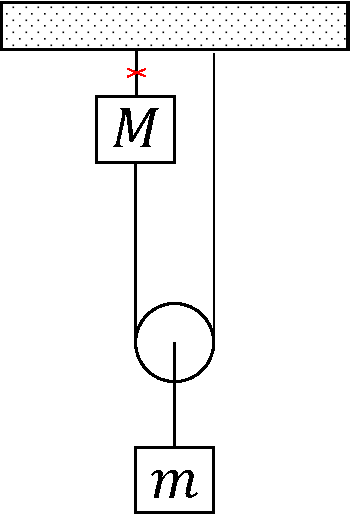
\includegraphics[width=0.6\linewidth]{2021-1/Imagenes/aux6/p3.pdf}
        \caption{P1}
    \end{subfigure}
    \begin{subfigure}[t]{0.4\textwidth}
        \svgpath{../../2021-1/Imagenes/aux7/}
        \centering
        \includesvg[width=1\linewidth]{p3.svg}
        \caption{P2}
    \end{subfigure}
\end{figure}


\item En presencia de la gravedad terrestre, una bolita de masa $m$ es sostenida mediante un resorte de constante elástica $k$ y longitud natural $L$, como se muestra en la figura. El conjunto se dispone dentro de un tubo de paredes lisas inclinado en un ángulo $\beta$ con respecto a la vertical. El tubo se hace girar con velocidad angular constante $\omega$ y la bolita mantiene una trayectoria circunferencial. El extremo superior $Q$ del resorte se ubica en el eje de rotación. Determine la elongación $\Delta$ del resorte y discuta la posibilidad de que $\Delta = 0$

\begin{figure}[H]
    \centering
    \includesvg[width=0.5\linewidth]{../../2021-1/Imagenes/aux9/resorte1.svg}
\end{figure}


\item Un bloque de masa $m$ se deja caer por un plano sin roce inclinado en un ángulo $\theta$. Cuando el bloque alcanza el final del plano, se desliza sobre una cinta que se mueve con rapidez $v_b$. Sea $\mu_k$ y $\mu_s$ los coeficientes de roce cinético y estático, respectivamente, de la cinta

\begin{enumerate}
    \item Determine el trabajo realizado por el peso
    
    \item Utilizando la parte anterior, determine la rapidez del bloque al llegar al final del plano
    
    \item Determine la distancia $d$ que recorre el bloque a lo largo de la cinta para que alcance la misma rapidez de esta.
    
    ¿Qué pasa si la rapidez calculada en la parte (b) es menor? ¿mayor? Separe ambas situaciones
\end{enumerate}

\begin{figure}[H]
    \centering
    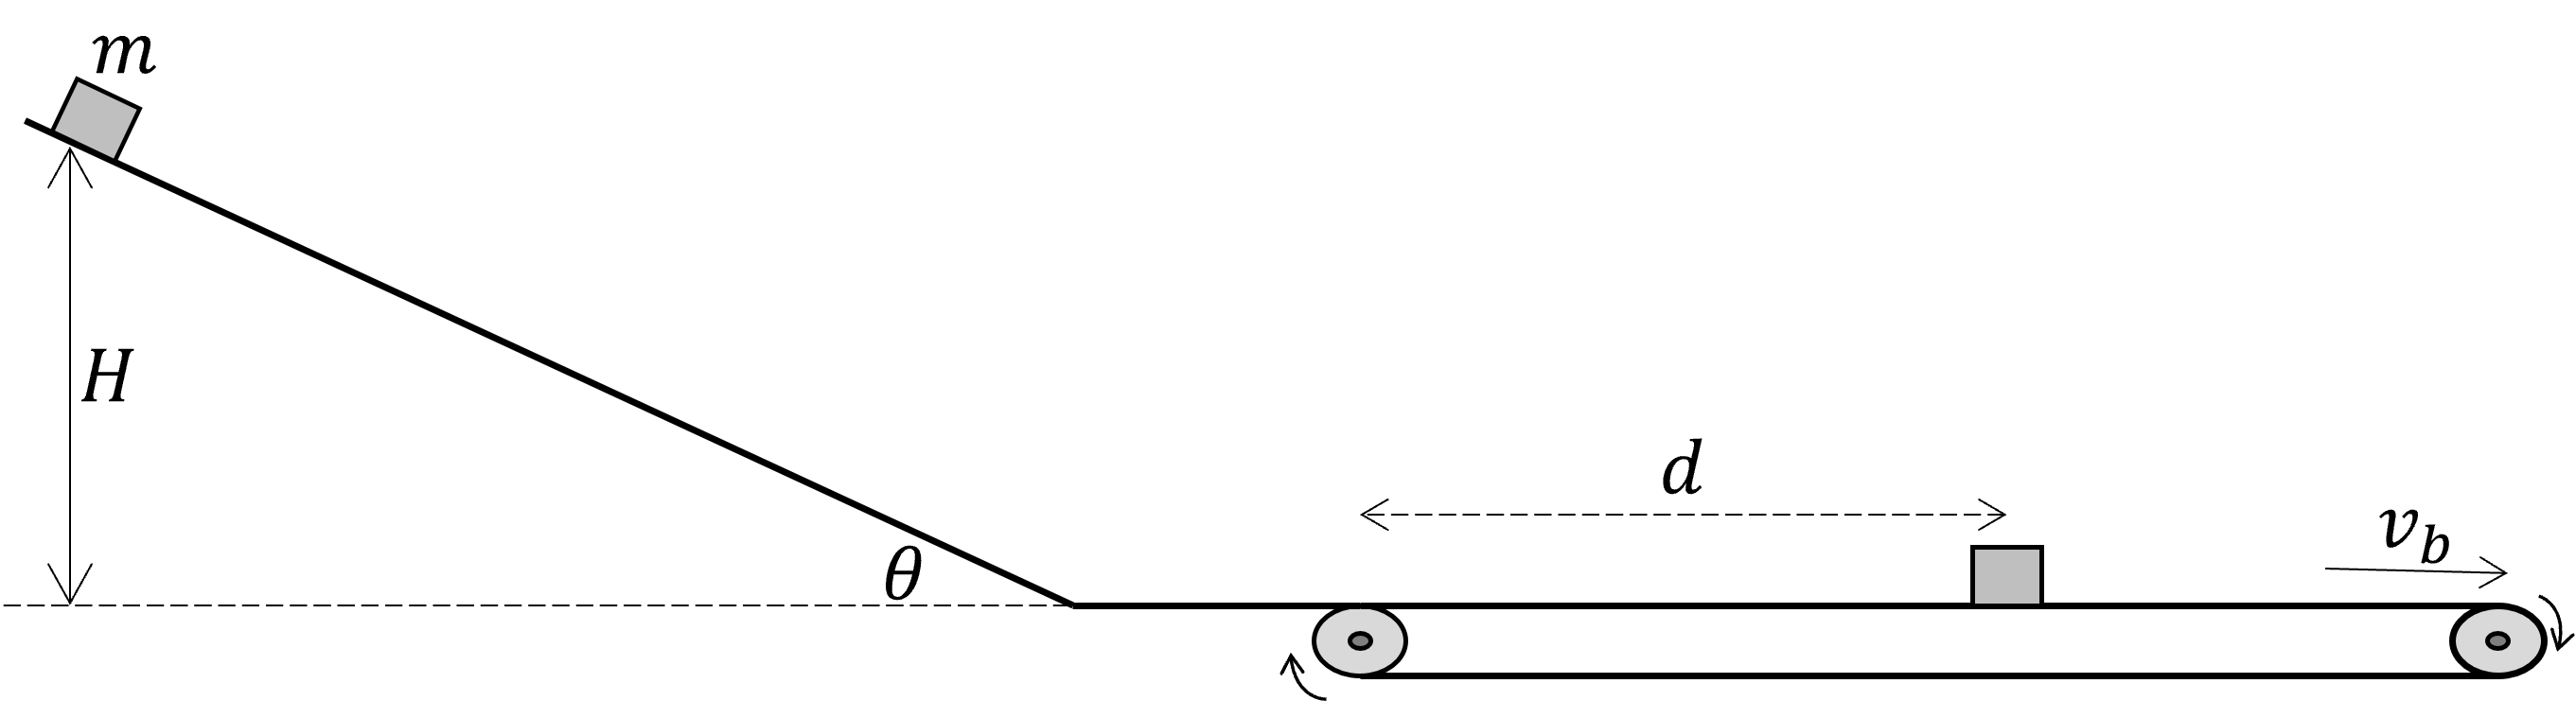
\includegraphics[width=0.8\linewidth]{2023-1/img/TD 3/cinta.png}
\end{figure}


% Para imágenes vectoriales -> el texto tiene que estar en LaTeX
% \begin{figure}[htbp]
%   \centering
%   \svgpath{../Imagenes/ejercicios}  -> .. irse pa'trás 
%   \includesvg{ej5.svg}
% \end{figure}

\end{enumerate}
\end{document}
